\normalfont \large Decades have passed since electric circuits become integrated on microchips or ICs. Technology is passing with time and now it is the time for photonics to get integrated into circuits. These can lead to a revolution in the digital technology we know today, with every hand-held device to corporate machines, all running on circuits made using photonic crystals and microresonators. 
\subparagraph{\normalfont \large These topics require a detailed study, which is what we are going to do in this Thesis. The research of this Thesis is centered towards devices such as microring resonators (I will discuss them later), which includes gain medium.}
\subparagraph{\normalfont \large This documentation is divided into different sections, compiling the work of 1 year long BS project. First, we will increase the understanding of the reader of what resonators, optical resonators, and microring resonators are. Then the study will focus on the systems that we used and their explanations, after that I will show the results of what I have collected by modeling the system in different conditions (parameters). This extensive documentation will be useful for anyone trying to get started in this field of research because I have written it in a fashion that a newbie in the field of photonics can easily grasp the ideas and can learn from it. }
\newpage
\section{Resonators}
\normalfont \large A resonator is a device that exhibits resonant behavior naturally (or artificially) on some resonant frequencies, that is, it oscillates at those frequencies with higher amplitudes than others. These frequencies are called its resonant frequencies. These oscillations can either be electromagnetic waves or mechanical waves as well. 
There are different uses of resonators, they can be used to filter some specific frequencies or can also be used to generate a specific frequency of the wave. A resonator in which the waves exists in hallow space is called a cavity resonator, which is used in electronics and radio signal processing,  known as microwave cavities, to generate, transmit and receive electromagnetic signals.  Acoustic cavity resonators, in which sound is produced by air vibrating in a cavity with one opening, are known as Helmholtz resonators.
\subsection{Explaination}
The term resonator is most often used for a homogeneous object in which vibrations travel as waves, at an approximately constant velocity, bouncing back and forth between the sides of the resonator. The material of the resonator, through which the waves flow, can be viewed as being made of millions of coupled moving parts (such as atoms). Therefore, they can have millions of resonant frequencies, although only a few may be used in practical resonators. The oppositely moving waves interfere with each other, and at its resonant frequencies reinforce each other to create a pattern of standing waves in the resonator. If the distance between the sides is ${\displaystyle d\,}$, the length of a round trip is ${\displaystyle 2d\,}$. To cause resonance, the phase of a sinusoidal wave after a round trip must be equal to the initial phase so the waves self-reinforce. The condition for resonance in a resonator is that the round trip distance, ${\displaystyle 2d\,}$, is equal to an integer number of wavelengths ${\displaystyle \lambda \,}$ of the wave:

$${\displaystyle 2d=N\lambda ,\qquad \qquad N\in \{1,2,3,\dots \}}$$

If the velocity of a wave is ${\displaystyle c\,}$, the frequency is ${\displaystyle f=c/\lambda \,}$ so the resonant frequencies are:

$${\displaystyle f={\frac {Nc}{2d}}\qquad \qquad N\in \{1,2,3,\dots \}}$$

So the resonant frequencies of resonators, called normal modes, are equally spaced multiples (harmonics) of a lowest frequency called the fundamental frequency. The above analysis assumes the medium inside the resonator is homogeneous, so the waves travel at a constant speed, and that the shape of the resonator is rectilinear. If the resonator is inhomogeneous or has a nonrectilinear shape, like a circular drumhead or a cylindrical microwave cavity, the resonant frequencies may not occur at equally spaced multiples of the fundamental frequency. They are then called overtones instead of harmonics. There may be several such series of resonant frequencies in a single resonator, corresponding to different modes of vibration.

\section{Optical Resonators}
An optical resonator, also known as optical cavity, is usually composed of two highly reflecting mirror held infront of each other parallely inside a vacum so that the system exhibits resonant behavior which allows standing wave modes to exist with almost no loss. Thus optical resonantor is a cavity with walls that are highly reflected for electromagnetic waves (i-e light).

\begin{figure}[h]
\centering
\reflectbox{%
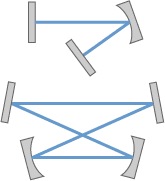
\includegraphics[scale=0.75]{linear_and_ring_resonator.png}}
\caption{Illustration of a basic optical cavity}
\end{figure}

\section{Micro Resonators}
Microresonators are special type of resonators made from different type of materials which exhibits optical properties while being fabricated on a chip. These kind of resonators are actually useful in observing the effects of optical resonators on a device.
\subsection{Different Geometeries}
There are many type of microresonators from which microring-resonators are very useful in making photonic devices and have wide variety of application. (See figure 1.2)
\begin{figure}[h]
\centering
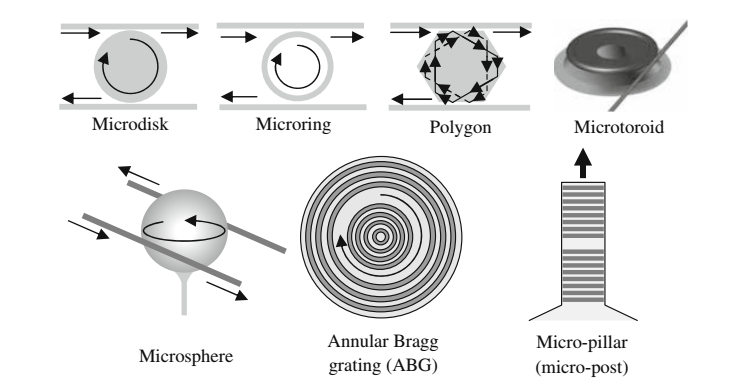
\includegraphics[width=1\textwidth]{microresonators_types.jpg}
\caption{Different geometeries of microresonators.}
\end{figure}

\subsection{All-Pass}
A straightforward ring resonator is made by taking one yield of a conventional directional coupler and bolstering it once again into one input. Such a device displays periodic cavity resonance (reverberation) when light navigating the ring procures a phase move relating to a number numerous of 2$\pi$ radians. The resonator is numerically defined from two parts: a coupling quality and an input way. In opposition to the limitless entirety inferences performed before for the Fabry– Perot and Gires– Tournois, in which we expected steadystate task and coordinating fields and derived basic spectral properties. Although, both strategies are similarly substantial, the field-coordinating technique has the benefit of simplicity.
\begin{figure}[h]
\centering
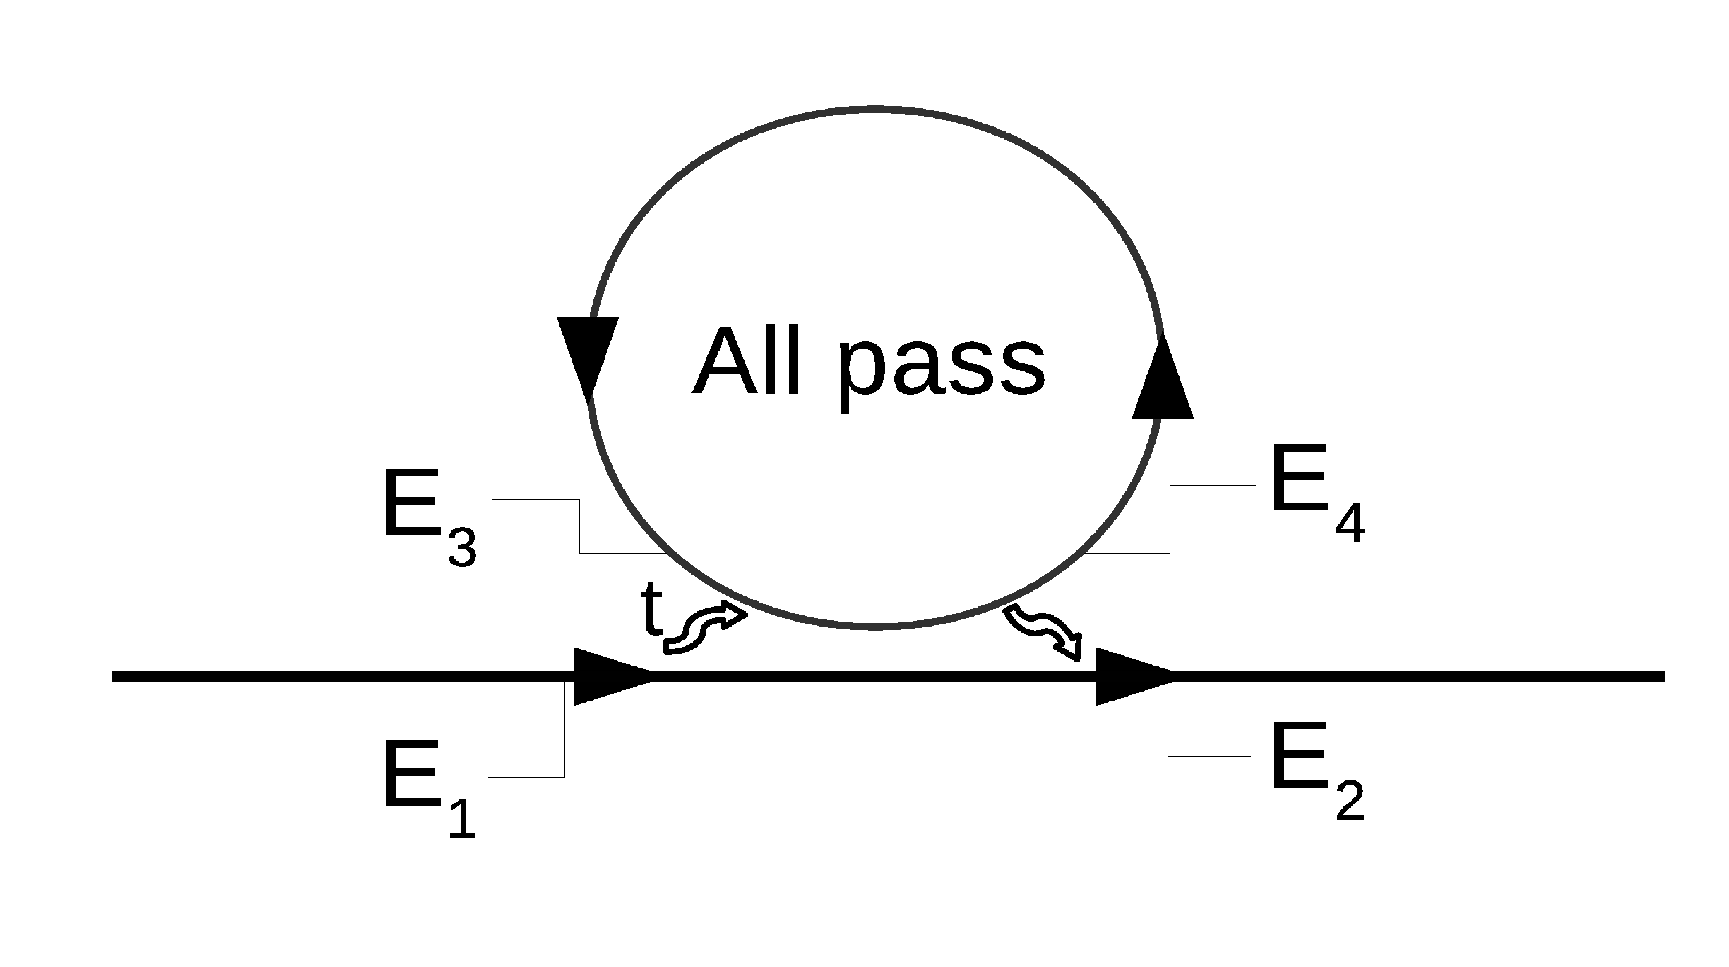
\includegraphics[width=0.5\textwidth]{all_pass_resonator.eps}
\caption{Illustrated fields of an all pass resonator}
\end{figure}
\subsection{Add drop}
The immediate waveguide similarity of a free-space Fabry– Perot is gotten by including a second guide that side-couples to the resonator as in Fig. 1.4.
Since this setup acts as a tight band abundancy channel that can include or drop a recurrence band from an approaching sign, it is regularly named an add– drop filter.
\begin{figure}[h]
\centering
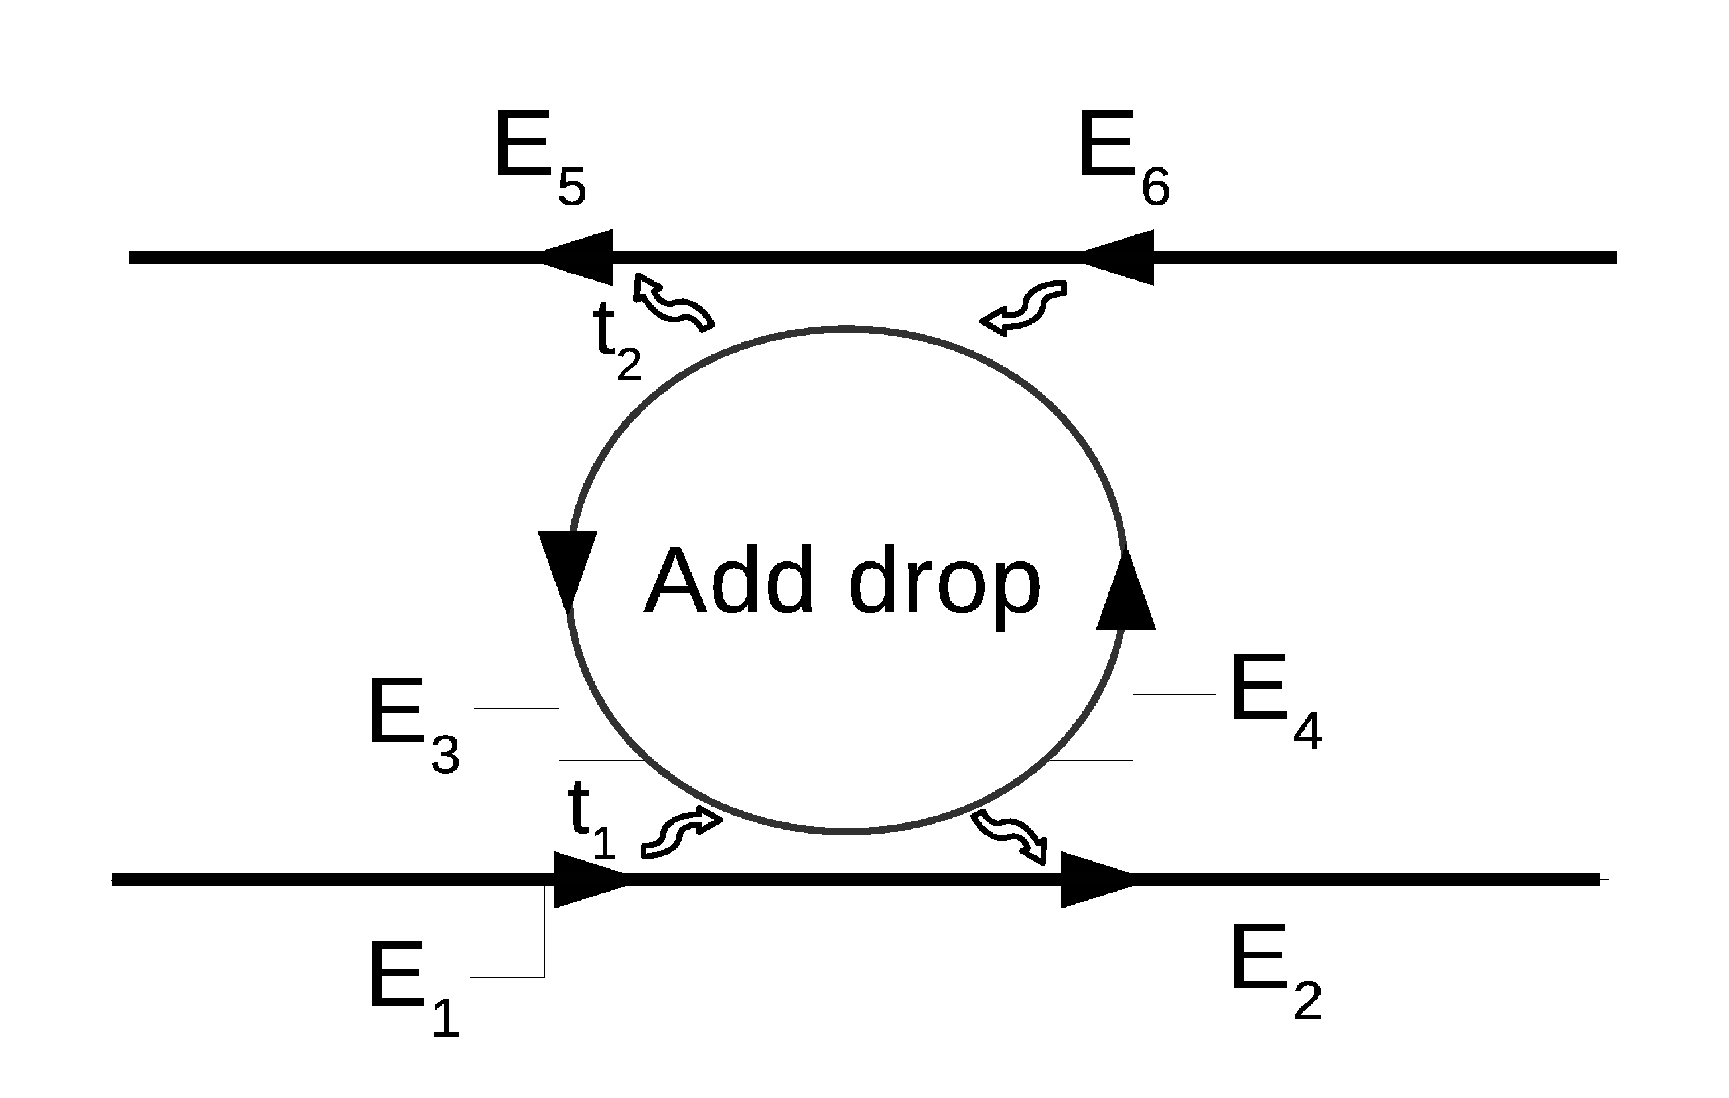
\includegraphics[width=0.75\textwidth]{add_drop_resonator.eps}
\caption{Illustrated fields of an add drop resonator}
\end{figure}
\subsection{Coupled Ring Resonator}
A simple case as an assymeteric Fabry-Perot resonator, a coupled ring resonator has another ring above the first ring of the all pass resonator. This arrangement shows coupling between the two resonators (rings) and show different behaviour. 
\begin{figure}[h]
\centering
\includegraphics[width=0.75\textwidth]{couple_ring_resonator.eps}
\caption{Illustrated fields and geometry of a coupled ring resonator}
\end{figure}

\newpage
\section*{References}
\addcontentsline{toc}{section}{References}

To perform more advanced calculations, it is important to have some understanding of how mpmath works internally and what the possible sources of error are. This section gives an overview of arbitrary-precision binary floating-point arithmetic and some concepts from numerical analysis.
To perform more advanced calculations, it is important to have some understanding of how mpmath works internally and what the possible sources of error are. This section gives an overview of arbitrary-precision binary floating-point arithmetic and some concepts from numerical analysis.
